% =============================================================================
% Module 1d: Geodesics and Orbits in Schwarzschild Spacetime
% =============================================================================
% Sources: Carroll Ch. 5 (Secs. 5.4--5.5), Congdon & Keeton Ch. 3.3.3
% Mathematica: ../Mathematica/01d_Geodesics_Orbits/
% =============================================================================

\chapter{Geodesics and Orbits in Schwarzschild Spacetime}
\label{ch:geodesics_orbits}

\begin{quote}
\textit{Together the conserved quantities $E$ and $L$ provide a convenient way
to understand the orbits of particles in the Schwarzschild geometry.}
\hfill --- Sean Carroll, \textit{Spacetime and Geometry}
\end{quote}

\noindent
In Module~1c we derived the Schwarzschild metric.  Now we ask: how do
particles and light \textit{move} in this spacetime?  The answer comes from
the geodesic equation, which we reduce to a one-dimensional effective
potential problem using Killing vectors and conservation laws.  This
module derives the effective potential for massive and massless particles,
identifies the key features (ISCO, photon sphere), and culminates in
Mercury's perihelion precession --- one of the three classical tests of GR.

\medskip
\noindent
\textbf{Companion Mathematica files:}
\begin{itemize}[nosep]
    \item \mathlink{01d_Geodesics_Orbits/geodesic_equation.wl}{geodesic\_equation.wl}
          --- symbolic derivation of the geodesic equations, conserved
          quantities, effective potential, ISCO, photon sphere, and
          perihelion precession formula
    \item \mathlink{01d_Geodesics_Orbits/effective_potential.nb}{effective\_potential.nb}
          --- interactive plots of effective potential with sliders for
          $L$ and $\epsilon$; orbit integration; precessing ellipses
\end{itemize}


% =====================================================================
\section{Killing Vectors and Conservation Laws}
\label{sec:killing_vectors}

The Schwarzschild metric is independent of both $t$ and $\phi$, which
means it possesses two \textbf{Killing vectors} (Carroll Sec.~5.4):
\begin{equation}
    K^\mu = (\partial_t)^\mu = (1, 0, 0, 0) \quad \text{(time translation)},
    \label{eq:killing_t}
\end{equation}
\begin{equation}
    R^\mu = (\partial_\phi)^\mu = (0, 0, 0, 1) \quad \text{(axial rotation)}.
    \label{eq:killing_phi}
\end{equation}
For any geodesic $x^\mu(\lambda)$, the quantity $K_\mu\, dx^\mu/d\lambda$
is conserved along the path (Carroll eq.~5.54).  Lowering the index with
the metric gives the two conserved quantities (Carroll eqs.~5.61--5.62):
\begin{equation}
    \boxed{
    E = \left(1 - \frac{R_S}{r}\right) \frac{dt}{d\lambda}
    }
    \label{eq:conserved_E}
\end{equation}
\begin{equation}
    \boxed{
    L = r^2 \frac{d\phi}{d\lambda}
    }
    \label{eq:conserved_L}
\end{equation}
For massive particles ($\lambda = \tau$), $E$ and $L$ are the conserved
energy and angular momentum \textit{per unit mass}.  For photons, they are
the energy and angular momentum of the photon (up to normalization of the
affine parameter).

Additionally, spherical symmetry allows us to restrict all orbits to the
equatorial plane $\theta = \pi/2$ without loss of generality (Carroll
eq.~5.56).


% =====================================================================
\section{The Effective Potential}
\label{sec:effective_potential}

The normalization condition for the four-velocity gives
(Carroll eq.~5.63):
\begin{equation}
    -\left(1 - \frac{R_S}{r}\right)\left(\frac{dt}{d\lambda}\right)^2
    + \left(1 - \frac{R_S}{r}\right)^{-1}\left(\frac{dr}{d\lambda}\right)^2
    + r^2\left(\frac{d\phi}{d\lambda}\right)^2 = -\epsilon \,,
    \label{eq:normalization}
\end{equation}
where $\epsilon = 1$ for massive particles (timelike geodesics) and
$\epsilon = 0$ for photons (null geodesics).

Substituting the conserved quantities~\eqref{eq:conserved_E}
and~\eqref{eq:conserved_L}, we obtain a radial equation
(Carroll eq.~5.64):
\begin{equation}
    \frac{1}{2}\left(\frac{dr}{d\lambda}\right)^2 + V_{\mathrm{eff}}(r)
    = \mathcal{E} \,,
    \label{eq:radial_equation}
\end{equation}
where the \textbf{effective potential} is (Carroll eq.~5.66;
Congdon \& Keeton eq.~3.80):
\begin{equation}
    \boxed{
    V_{\mathrm{eff}}(r) = -\epsilon\,\frac{GM}{r}
    + \frac{L^2}{2r^2}
    - \frac{GML^2}{c^2 r^3}
    }
    \label{eq:effective_potential}
\end{equation}
and $\mathcal{E} = \half(E^2 - \epsilon c^2)$ is the effective ``energy.''

\begin{remark}
The three terms in $V_{\mathrm{eff}}$ have clear physical interpretations:
\begin{enumerate}[nosep]
    \item $-\epsilon\, GM/r$: the Newtonian gravitational potential
          (absent for photons since $\epsilon = 0$)
    \item $L^2/(2r^2)$: the centrifugal barrier (identical to Newtonian
          mechanics)
    \item $-GML^2/(c^2 r^3)$: the \textbf{GR correction} --- this term
          has no Newtonian analogue and is responsible for all the
          distinctive features of relativistic orbits
\end{enumerate}
The GR term is attractive at small $r$, which means the centrifugal
barrier can be overcome --- this is why particles can spiral into black
holes, which is impossible in Newtonian gravity.
\end{remark}

\begin{figure}[ht]
    \centering
    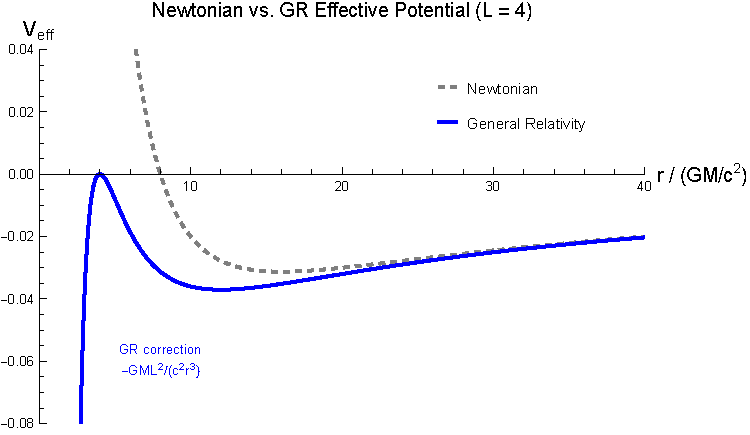
\includegraphics[width=0.75\textwidth]{../Figures/01d_Geodesics_Orbits/newtonian_vs_gr.pdf}
    \caption{Comparison of Newtonian (dashed) and GR (solid) effective
    potentials for a massive particle with $L = 4\,GM/c$.  The GR correction
    term $\propto 1/r^3$ pulls the potential down at small $r$, allowing
    particles to plunge past the centrifugal barrier.
    (cf.\ Carroll Figs.~5.4 and 5.5)}
    \label{fig:newtonian_vs_gr}
\end{figure}


% =====================================================================
\section{Circular Orbits and the ISCO}
\label{sec:circular_orbits}

Circular orbits occur at extrema of the effective potential:
$dV_{\mathrm{eff}}/dr = 0$.  For massive particles ($\epsilon = 1$),
this gives (Carroll eq.~5.68):
\begin{equation}
    GM r_c^2 - L^2 r_c + 3GML^2/c^2 = 0 \,.
    \label{eq:circular_condition}
\end{equation}
The two solutions are (Carroll eq.~5.71):
\begin{equation}
    r_\pm = \frac{L^2}{2GM}
    \left(1 \pm \sqrt{1 - \frac{12G^2M^2}{L^2 c^2}}\right) \,.
    \label{eq:circular_radii}
\end{equation}

\begin{itemize}
    \item $r_+$ (outer): \textbf{stable} circular orbit (minimum of $V_{\mathrm{eff}}$)
    \item $r_-$ (inner): \textbf{unstable} circular orbit (maximum of $V_{\mathrm{eff}}$)
\end{itemize}

Real solutions require $L^2 \geq 12\,G^2M^2/c^2$, i.e.,
$L \geq 2\sqrt{3}\,GM/c$ (Carroll eq.~5.73).  The minimum stable circular
orbit occurs when $r_+ = r_-$, giving the \textbf{innermost stable
circular orbit (ISCO)} (Carroll eq.~5.74; Congdon \& Keeton eq.~3.84):
\begin{equation}
    \boxed{r_{\mathrm{ISCO}} = \frac{6GM}{c^2} = 3\, R_S}
    \label{eq:ISCO}
\end{equation}

\begin{remark}
The ISCO is a fundamental scale in black hole astrophysics.  Accreting
matter in a thin disk spirals inward until it reaches the ISCO, then
plunges into the black hole.  The ISCO radius determines the
efficiency of energy extraction from accretion and the inner edge of
accretion disks observed in X-ray binaries and active galactic nuclei.
\end{remark}


% =====================================================================
\section{The Photon Sphere}
\label{sec:photon_sphere}

For photons ($\epsilon = 0$), the effective potential simplifies to
(Congdon \& Keeton eq.~3.86):
\begin{equation}
    V_{\mathrm{eff}}^{\mathrm{photon}}(r) = \frac{L^2}{2r^2}
    - \frac{GML^2}{c^2 r^3} \,.
    \label{eq:Veff_photon}
\end{equation}
Setting $dV_{\mathrm{eff}}/dr = 0$ gives a single circular orbit
(Carroll eq.~5.70; Congdon \& Keeton eq.~3.84 with $\ell_{\mathrm{crit}}$):
\begin{equation}
    \boxed{r_{\mathrm{photon}} = \frac{3GM}{c^2} = \frac{3}{2}\, R_S}
    \label{eq:photon_sphere}
\end{equation}
This is an \textit{unstable} circular orbit --- any perturbation causes
the photon to either escape to infinity or spiral into the black hole.
Nevertheless, the photon sphere plays a key role in strong gravitational
lensing near black holes and is directly related to the ``photon ring''
observed by the Event Horizon Telescope.


% =====================================================================
\section{Effective Potential: Newtonian vs.\ GR}
\label{sec:veff_comparison}

The key qualitative differences between Newtonian and GR effective
potentials are:

\begin{center}
\begin{tabular}{lcc}
\toprule
\textbf{Feature} & \textbf{Newtonian} & \textbf{GR} \\
\midrule
Centrifugal barrier & Diverges as $r \to 0$ & Overcome at small $r$ \\
ISCO & None (stable at any $r$) & $r = 3R_S$ \\
Photon orbits & None & Unstable at $r = 3R_S/2$ \\
Plunge orbits & Impossible & Possible for $r < r_{\mathrm{ISCO}}$ \\
\bottomrule
\end{tabular}
\end{center}

\begin{figure}[ht]
    \centering
    \begin{subfigure}[b]{0.48\textwidth}
        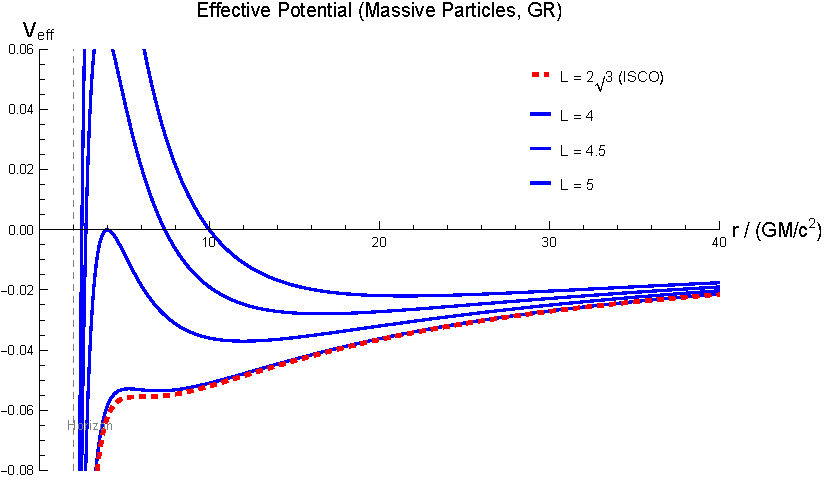
\includegraphics[width=\textwidth]{../Figures/01d_Geodesics_Orbits/effective_potential_massive.pdf}
        \caption{Massive particles ($\epsilon = 1$)}
    \end{subfigure}
    \hfill
    \begin{subfigure}[b]{0.48\textwidth}
        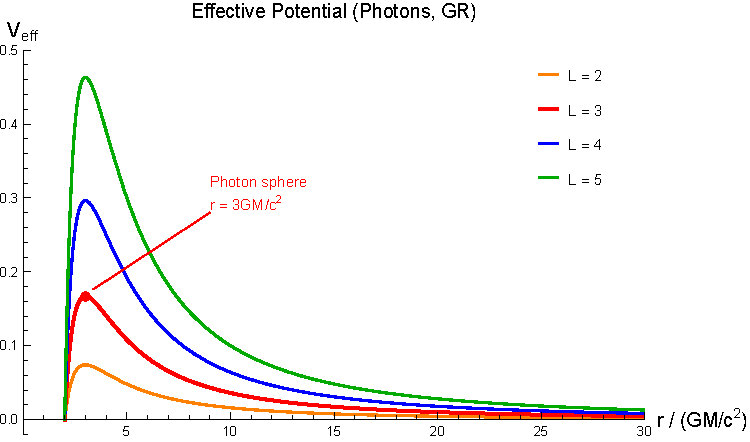
\includegraphics[width=\textwidth]{../Figures/01d_Geodesics_Orbits/effective_potential_photon.pdf}
        \caption{Photons ($\epsilon = 0$)}
    \end{subfigure}
    \caption{GR effective potentials for several values of angular momentum
    $L$ (in $GM/c$ units).  \textbf{Left:} For massive particles, the red
    dashed curve shows $L = L_{\mathrm{ISCO}} = 2\sqrt{3}\,GM/c$, where
    the stable and unstable circular orbits merge.  \textbf{Right:} For
    photons, the potential always has a maximum at $r = 3GM/c^2$ (the photon
    sphere).  Interactive versions in
    \texttt{effective\_potential.nb}.}
    \label{fig:effective_potentials}
\end{figure}


% =====================================================================
\section{Perihelion Precession}
\label{sec:perihelion_precession}

In Newtonian gravity, bound orbits are perfect ellipses that close on
themselves.  In GR, the extra $-GML^2/(c^2 r^3)$ term in the effective
potential causes the orbit to \textit{precess}: the perihelion (point of
closest approach) advances by a small angle each orbit.

Following Carroll Sec.~5.5 and using the substitution $x = L^2/(GMr)$,
the orbit equation becomes (Carroll eq.~5.79):
\begin{equation}
    \frac{d^2 x}{d\phi^2} + x = 1 + \frac{3G^2M^2}{L^2 c^2}\, x^2 \,.
    \label{eq:orbit_equation}
\end{equation}
The last term is the GR correction.  Treating it as a perturbation
($x = x_0 + x_1$, with $x_0 = 1 + e\cos\phi$ the Keplerian solution),
one finds the accumulated precession per orbit
(Carroll eq.~5.92; Congdon \& Keeton eq.~3.95):
\begin{equation}
    \boxed{
    \Delta\phi = \frac{6\pi G M}{c^2 a(1 - e^2)}
    = \frac{6\pi G M}{L^2 / (GM)}
    }
    \label{eq:perihelion_precession}
\end{equation}
where $a$ is the semi-major axis and $e$ the eccentricity.

For Mercury (Carroll eq.~5.96):
\begin{equation}
    \Delta\phi_{\mathrm{Mercury}} = 5.01 \times 10^{-7}~\text{rad/orbit}
    = 0.103''\text{/orbit} = 43.0''\text{/century} \,.
    \label{eq:mercury_precession}
\end{equation}
This matched the previously unexplained 43~arcseconds/century discrepancy
in Mercury's orbit and was one of Einstein's first confirmations of GR.

\begin{figure}[ht]
    \centering
    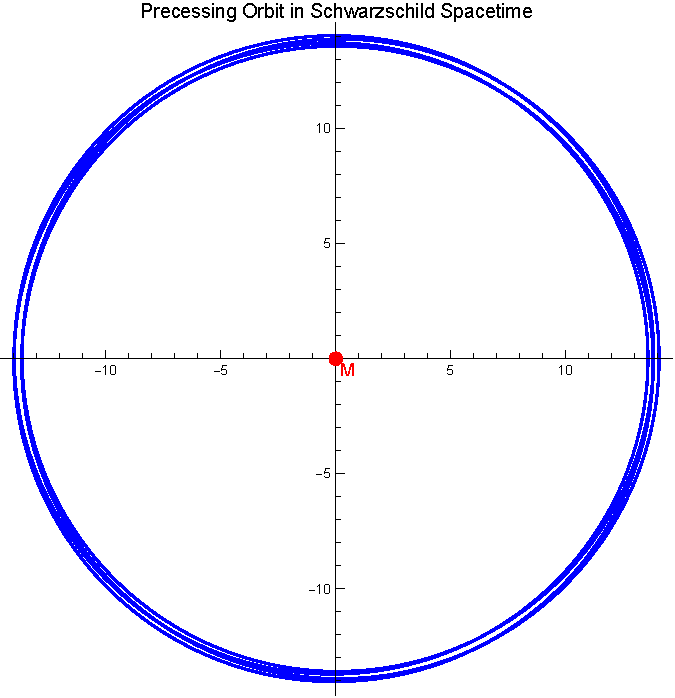
\includegraphics[width=0.55\textwidth]{../Figures/01d_Geodesics_Orbits/precessing_orbit.pdf}
    \caption{A precessing orbit in Schwarzschild spacetime, computed by
    numerically integrating the orbit equation.  The perihelion advances
    by a small angle each orbit, tracing out a rosette pattern.
    (cf.\ Carroll Fig.~5.6)}
    \label{fig:precessing_orbit}
\end{figure}


% =====================================================================
\section{Null Geodesics and the Deflection of Light (Preview)}
\label{sec:null_geodesics_preview}

For photons, the orbit equation (using $u = 1/r$) becomes
(Congdon \& Keeton eq.~3.87):
\begin{equation}
    \frac{d\phi}{dr} = \pm \frac{L}{r^2}
    \left[\frac{E^2}{c^2} - \frac{L^2}{r^2}\left(1 - \frac{R_S}{r}\right)
    \right]^{-1/2} \,.
    \label{eq:photon_orbit}
\end{equation}
A photon approaching a mass $M$ with impact parameter $b = cL/E$
(the perpendicular distance from the mass in the absence of deflection)
will be deflected by an angle (Congdon \& Keeton eq.~3.96):
\begin{equation}
    \hat{\alpha} = \frac{4GM}{c^2 b} \,,
    \label{eq:deflection_preview}
\end{equation}
in the weak-field limit ($b \gg R_S$).  This is \textit{twice} the
Newtonian prediction and was confirmed by Eddington's 1919 solar eclipse
observations.

The full derivation of the deflection angle is the subject of Module~2.
We mention it here because the effective potential framework makes it
clear \textit{why} light bends: photons follow null geodesics of the
curved Schwarzschild spacetime, and the GR correction term in the
effective potential deflects them more strongly than Newtonian gravity
would predict.


% =====================================================================
\section{Brief Overview: The Kerr Metric}
\label{sec:kerr_overview}

Real astrophysical black holes are not perfectly described by the
Schwarzschild solution because they \textit{rotate}.  The metric for a
rotating, axially symmetric black hole is the \textbf{Kerr metric},
discovered by Roy Kerr in 1963.  In Boyer--Lindquist coordinates, it
takes the form:
\begin{equation}
    ds^2 = -\left(1 - \frac{R_S r}{\Sigma}\right) c^2 dt^2
    - \frac{2R_S r a \sin^2\theta}{\Sigma}\, c\, dt\, d\phi
    + \frac{\Sigma}{\Delta}\, dr^2
    + \Sigma\, d\theta^2
    + \frac{A \sin^2\theta}{\Sigma}\, d\phi^2 \,,
    \label{eq:kerr_metric}
\end{equation}
where
\begin{align}
    \Sigma &= r^2 + a^2\cos^2\theta \,, &
    \Delta &= r^2 - R_S r + a^2 \,, &
    A &= (r^2 + a^2)^2 - a^2 \Delta \sin^2\theta \,,
    \label{eq:kerr_functions}
\end{align}
and $a = J/(Mc)$ is the \textbf{spin parameter} (angular momentum per
unit mass, with dimensions of length).  Note $0 \leq a \leq GM/c^2$
for a physical black hole.

Key features that differ from Schwarzschild:
\begin{itemize}
    \item \textbf{Frame dragging:} The $dt\,d\phi$ cross-term forces
          particles near the black hole to co-rotate.  This effect is
          absent in Schwarzschild.
    \item \textbf{Ergosphere:} The region $R_S/2 < r < (R_S + \sqrt{R_S^2 -
          4a^2\cos^2\theta})/2$ where even stationary observers must rotate
          with the black hole.
    \item \textbf{Spin-dependent ISCO:} The ISCO radius depends on the spin
          parameter and the direction of the orbit (prograde vs.\ retrograde).
          For a maximally spinning black hole ($a = GM/c^2$):
          $r_{\mathrm{ISCO}} = GM/c^2$ (prograde) vs.\
          $r_{\mathrm{ISCO}} = 9GM/c^2$ (retrograde), compared to
          $6GM/c^2$ for Schwarzschild.
    \item \textbf{Two horizons:}
          $r_\pm = GM/c^2 \pm \sqrt{(GM/c^2)^2 - a^2}$.
\end{itemize}

\begin{remark}
For gravitational lensing by galaxies and clusters, the Kerr metric is
not needed: the lensing effect is dominated by the total enclosed mass,
and the weak-field/thin-lens approximation (Module~1e and beyond) washes
out spin effects at the angular scales of interest.  However, Kerr lensing
is an active research topic for \textit{strong} lensing near individual
black holes --- for instance, the ``photon ring'' structure observed by
the Event Horizon Telescope, where frame-dragging produces asymmetric
brightness patterns.
\end{remark}


% =====================================================================
\section{Summary}
\label{sec:geodesics_summary}

\begin{itemize}
    \item Killing vectors ($\partial_t$, $\partial_\phi$) yield conserved
          energy $E$ and angular momentum $L$ along geodesics.
    \item The radial motion reduces to a 1D effective potential problem:
          $V_{\mathrm{eff}} = -\epsilon GM/r + L^2/(2r^2) - GML^2/(c^2 r^3)$.
    \item The GR correction term $\propto 1/r^3$ is responsible for:
          ISCO at $r = 3R_S$, photon sphere at $r = 3R_S/2$, perihelion
          precession, and enhanced light deflection.
    \item Mercury's perihelion precesses by 43 arcsec/century --- confirmed
          by observation and one of the first tests of GR.
    \item The Kerr metric generalizes Schwarzschild to rotating black holes
          (frame dragging, ergosphere, spin-dependent ISCO), but is not
          needed for galaxy/cluster-scale lensing.
\end{itemize}


% =====================================================================
\section{Problems}
\label{sec:geodesics_problems}

\begin{exercise}
\label{ex:derive_veff}
Starting from the normalization condition~\eqref{eq:normalization} and the
conserved quantities $E$ and $L$, derive the effective
potential~\eqref{eq:effective_potential} for massive particles
($\epsilon = 1$).  Show that in the Newtonian limit ($c \to \infty$,
$R_S \to 0$), it reduces to
$V_{\mathrm{eff}}^{\mathrm{Newton}} = -GM/r + L^2/(2r^2)$.
\end{exercise}

\begin{exercise}
\label{ex:isco_derivation}
Derive the ISCO radius by finding the value of $L$ for which the two
circular orbit solutions~\eqref{eq:circular_radii} coincide (i.e., the
discriminant vanishes).  Verify $r_{\mathrm{ISCO}} = 6GM/c^2 = 3R_S$.
\end{exercise}

\begin{exercise}
\label{ex:photon_sphere_derivation}
Show that the only circular photon orbit in the Schwarzschild spacetime is
at $r = 3GM/c^2 = 3R_S/2$, and that it is unstable (a maximum of
$V_{\mathrm{eff}}^{\mathrm{photon}}$).
\end{exercise}

\begin{exercise}
\label{ex:mercury_precession}
Compute the perihelion precession of Mercury using
eq.~\eqref{eq:perihelion_precession} with:
$M = M_\odot$, $a = 5.79 \times 10^{10}$~m, $e = 0.2056$.
Verify $\Delta\phi \approx 43''$/century (Mercury's orbital period is
87.97 days).
\end{exercise}

\begin{exercise}
\label{ex:orbit_integration}
Using the effective potential for massive particles with $L = 4GM/c$:
\begin{enumerate}[label=(\alph*)]
    \item Plot $V_{\mathrm{eff}}(r)$ and identify the stable circular
          orbit radius, the unstable circular orbit radius, and the
          ISCO.
    \item For a particle with $\mathcal{E}$ slightly above
          $V_{\mathrm{eff}}(r_+)$, describe qualitatively the type of
          orbit (bound precessing ellipse, scatter orbit, or plunge orbit).
\end{enumerate}
\end{exercise}
